\chapter{Grafos dirigidos}

Los grafos dirigidos son un caso especial en el que las aristas tienen la noción de dirección, es decir, estas conectan desde un vértice hacia otro. Por ejemplo, un grafo dirigido con dos vértices en el que hay una arista de A hacia B se ve de la siguiente forma:

\begin{center}
	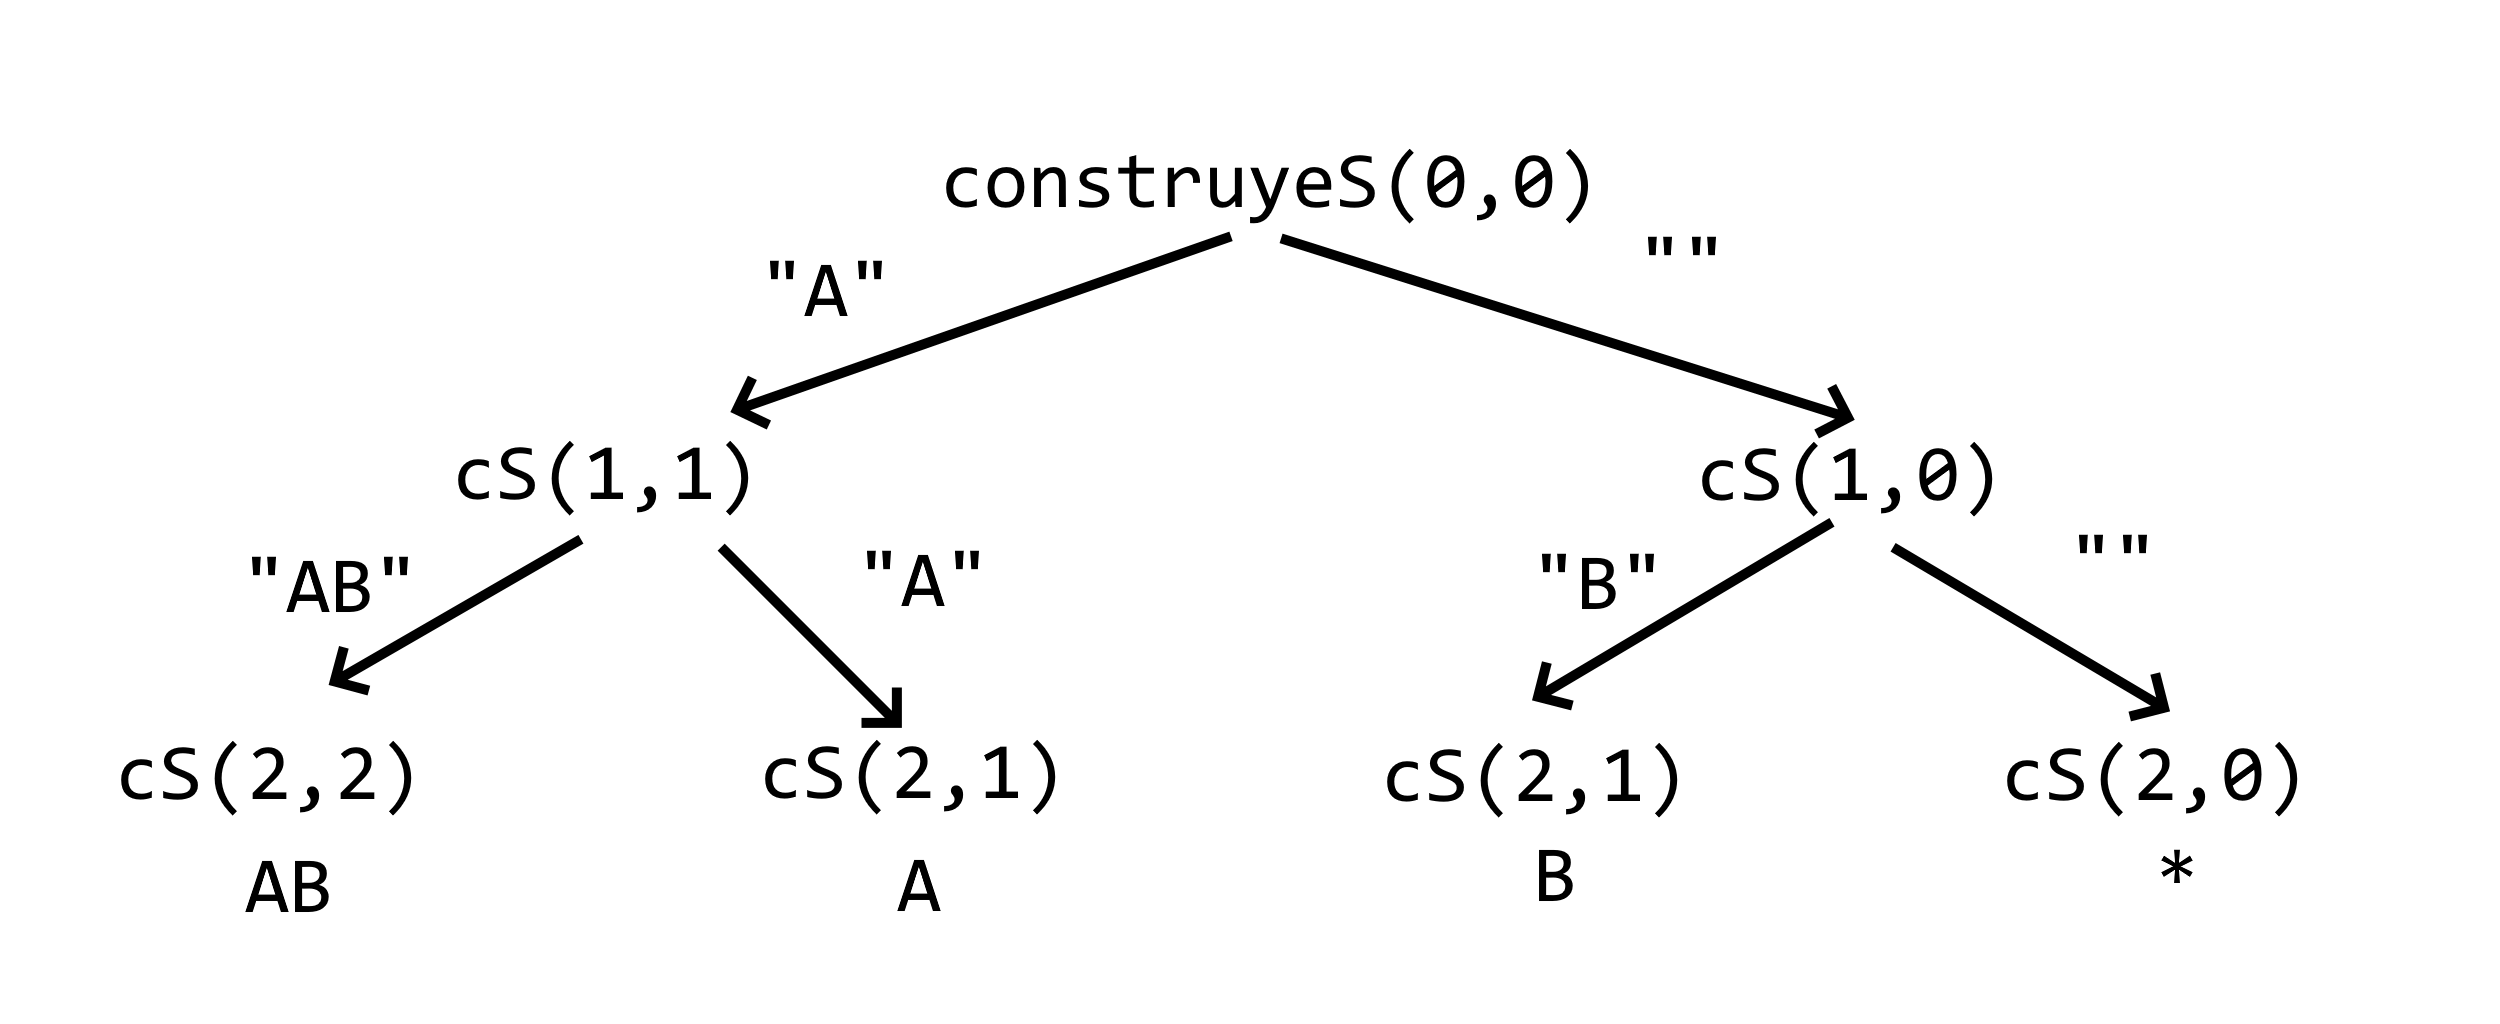
\includegraphics[scale=0.4]{grafos/dirigidos/AB}
\end{center}

Darle un sentido de orientación a las aristas resulta útil para muchos problemas en los que la relación tiene una dirección, orden o jerarquía. Por ejemplo, si los vértices representan personas y una arista significa que A le dio un regalo a B. Hay una persona que da y una que recibe.

\section{Grados}
A continuación explicaremos el concepto de grado en un grafo dirigido, que es ligeramente diferente a uno no dirigido.

\paragraph{Grado entrante:} El grado entrante (en inglés indegree) es el número de aristas que apuntan a un vértice. Por ejemplo, en el siguiente grafo el nodo C tiene grado entrante de 2, mientras que A y B tienen grado entrante de 0.

\begin{center}
	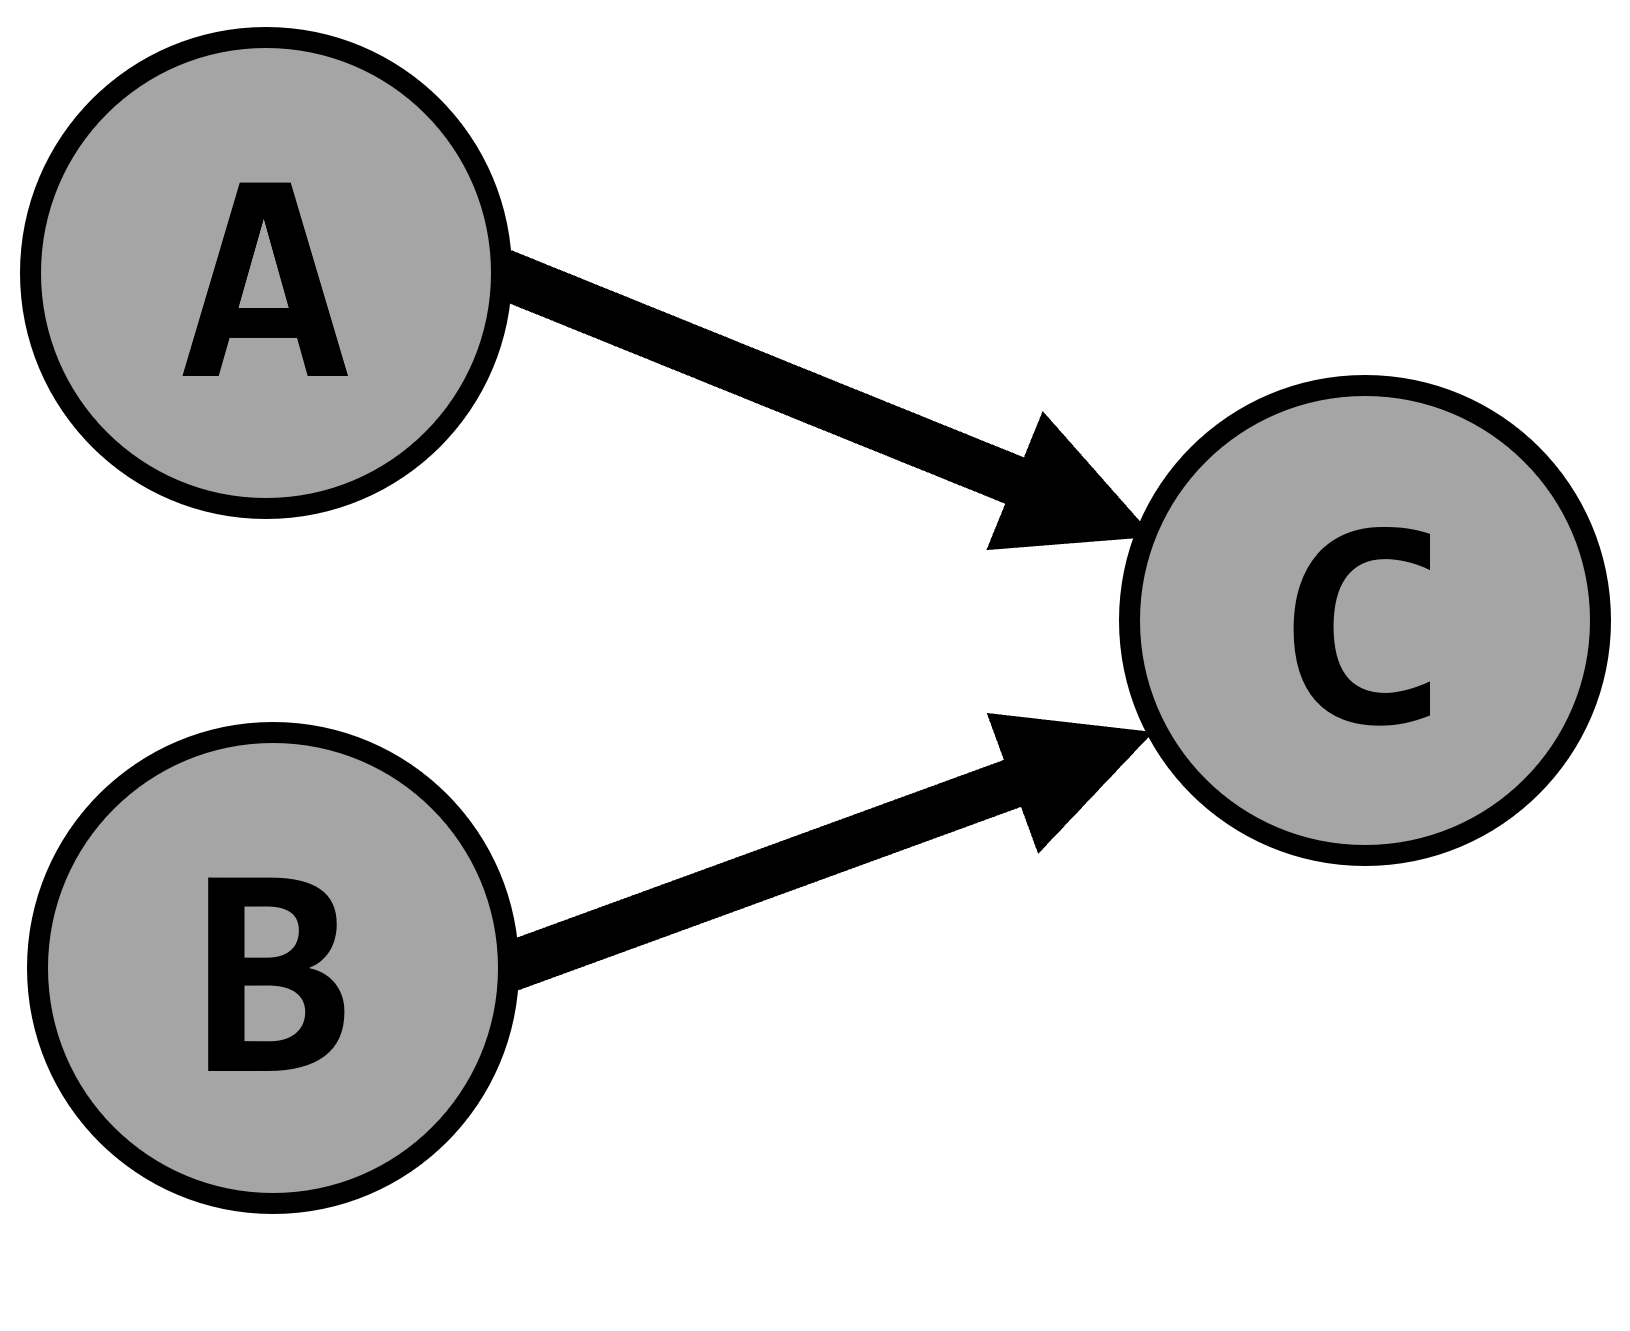
\includegraphics[scale=0.20]{grafos/dirigidos/indegree}
\end{center}

\paragraph{Grado saliente:} El grado saliente (en inglés outdegree) de un vértice es la cantidad de vértices aristas que salen desde este nodo y apuntan a otros. Por ejemplo En el siguiente ejemplo el nodo A tiene grado saliente de 2, mientras que los demás tienen 0.

\begin{center}
	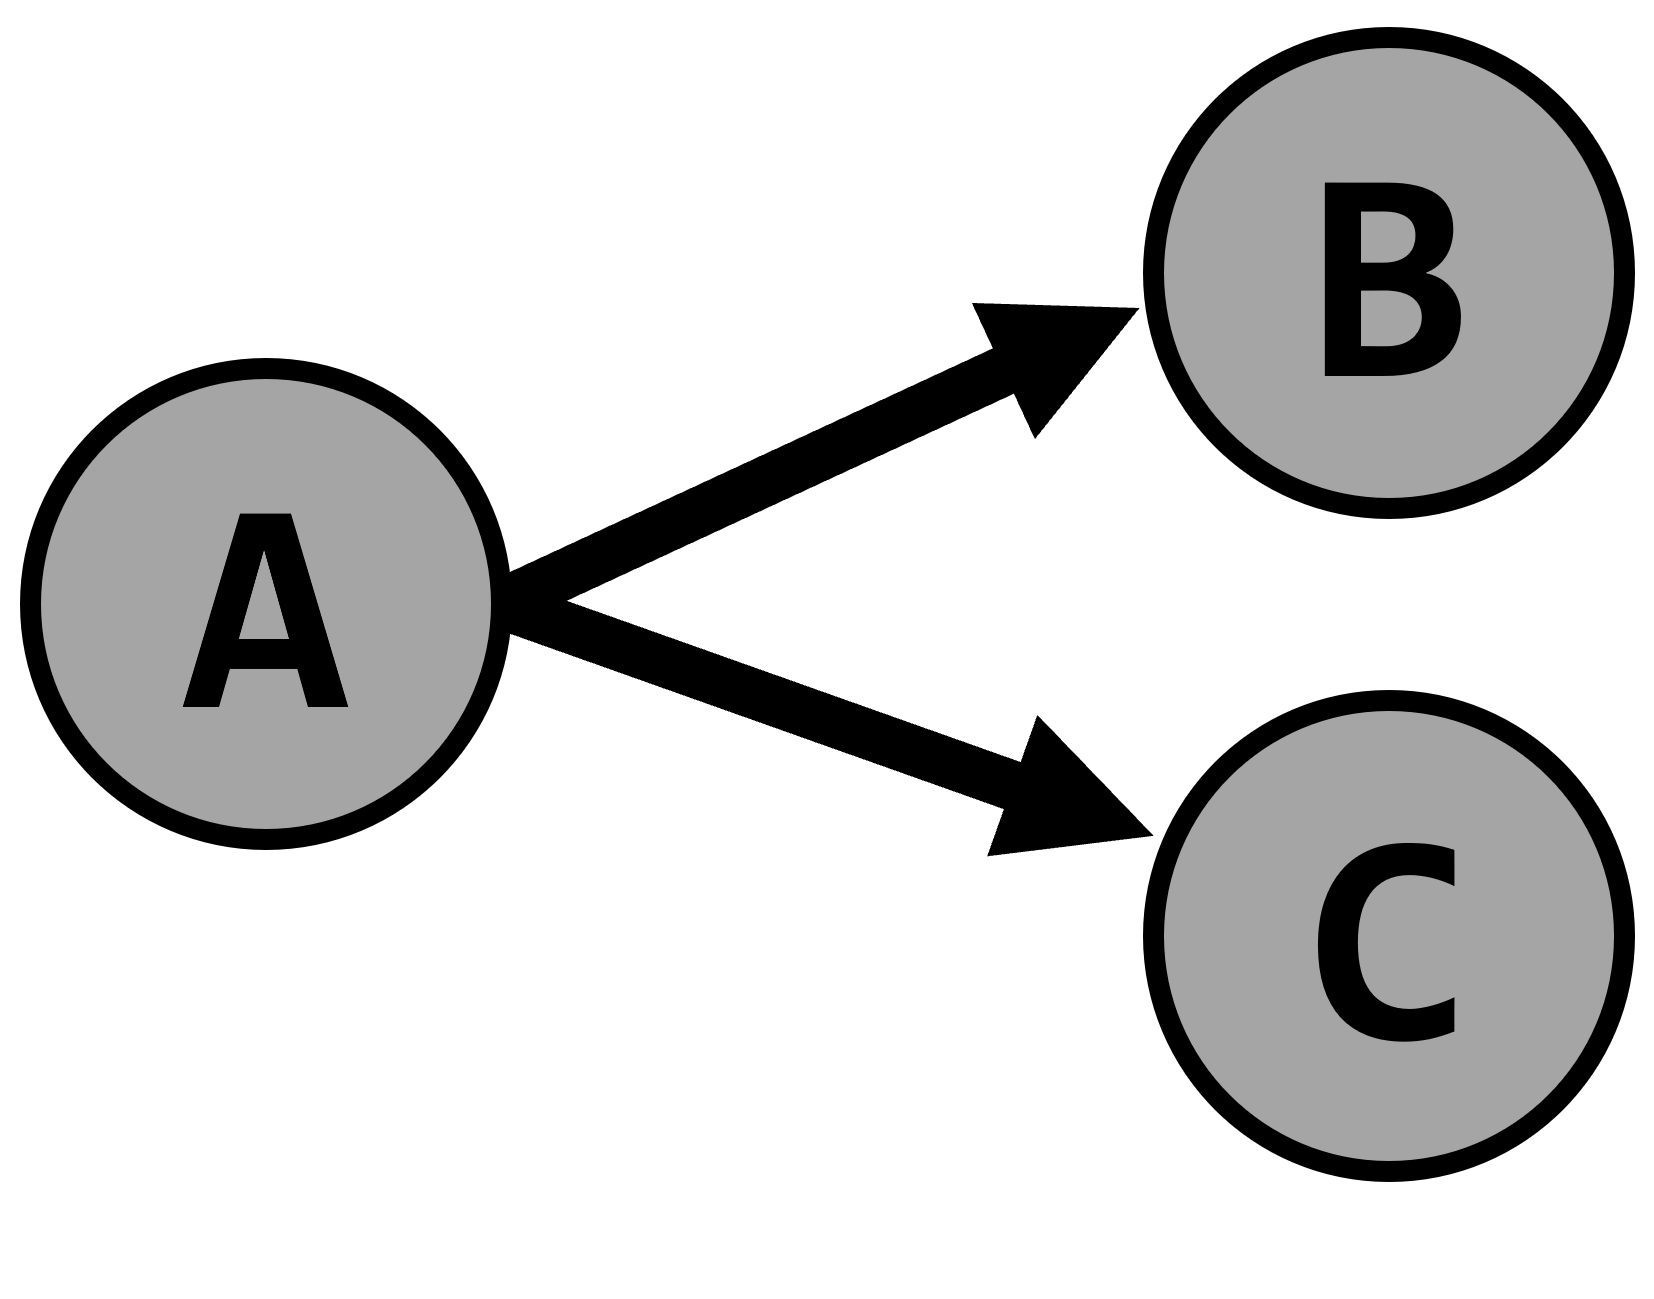
\includegraphics[scale=0.20]{grafos/dirigidos/outdegree}
\end{center}

\begin{exercise}
	\problema{Dar y recibir}{TODO} 
\end{exercise}

\section{Representación en memoria}
Los grafos dirigidos son representados en memoria de forma casi idéntica a los grafos que no son dirigidos. 

\subsection*{Matriz de adyacencia}
Si queremos representar un grafo dirigido con una matriz de adyacencia, entonces cada arista \(u \rightarrow v\) ocasionara que \verb|matriz[u][v] = 1|, pero NO debemos marcar el valor transpuesto de \verb|matriz[v][u]| si no existe la arista en dirección contraria.

Veamos la representación del siguiente grafo en una matriz de adyacencia.
\begin{center}
	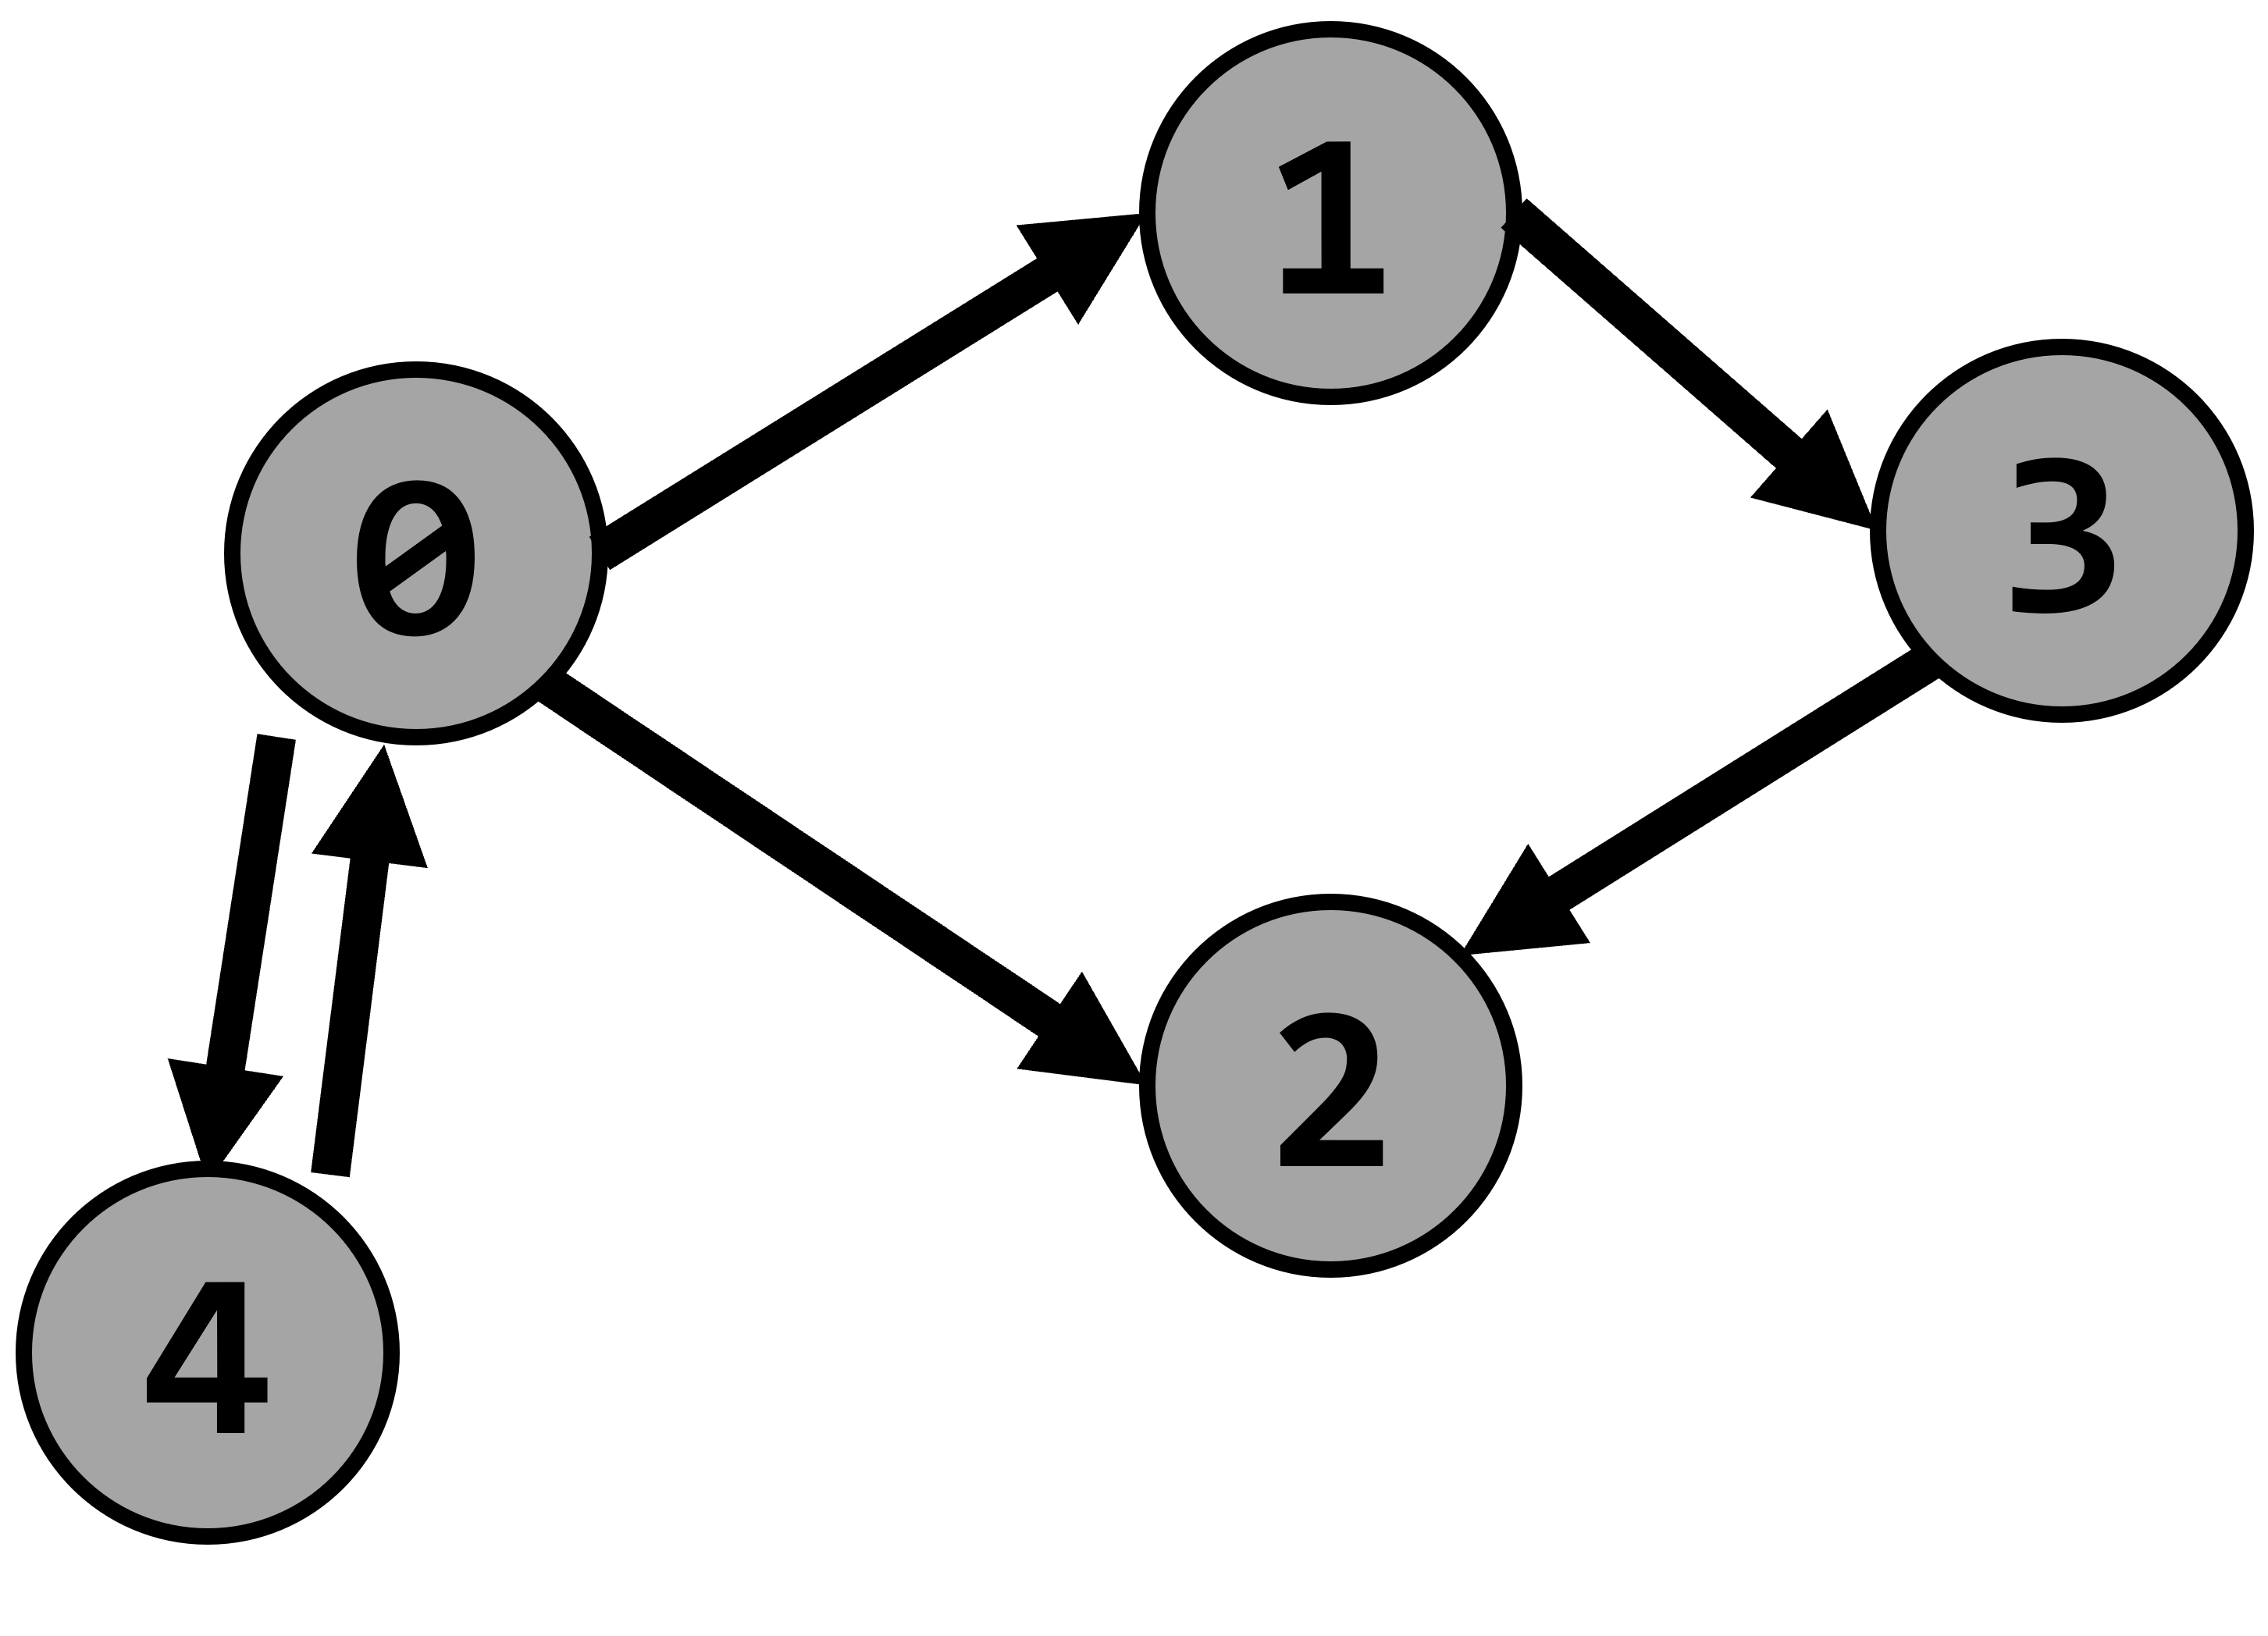
\includegraphics[scale=0.25]{grafos/dirigidos/ejemplo2}
\end{center}

La matriz de adyacencia es:
\begin{large}
	\begin{displaymath}	
		matriz = \begin{pmatrix}
			0 & 1 & 1 & 0 & 1\\
			0 & 0 & 0 & 1 & 0\\
			0 & 0 & 0 & 0 & 0\\
			0 & 0 & 1 & 0 & 0\\
			1 & 0 & 0 & 0 & 0
		\end{pmatrix}
	\end{displaymath}
\end{large}


\subsection*{Lista de adyacencia}
Igualmente, si tenemos que existe la arista \(u \rightarrow v\), entonces \(v\) aparecerá en \verb|listaAdyacencia[v]|, pero no implica que \(v\) aparezca en la lista de \(u\).

Las listas de adyacencia del grafo anterior quedan de la siguiente forma:
{
\begin{align*}
listaAdyacencia[0] & =\{1,4,2\} \\
listaAdyacencia[1] & =\{3\}\\
listaAdyacencia[2] & =\{\}\\
listaAdyacencia[3] & =\{2\}\\
listaAdyacencia[4] & =\{0\}
\end{align*}
}

\subsubsection*{Ejemplo: Cadena de regalos}
Fernando tiene \(N\) amigos enumerados del \(1\) al \(N\). Entre ellos existe la costumbre de dar regalos. Pero los amigos evitan gastar dinero cuando pueden y muchas veces tienden a regalar el mismo objeto que les fue obsequiado previamente.

Entonces, por ejemplo. Si el amigo 1 le regala una tetera a la persona 2, es perfectamente posible que después la persona 2 le regale esa misma tetera al amigo número 5. 

Fernando un día regalo por accidente un tesoro de su familia al amigo etiquetado 1 y ahora quiere recuperarlo. Pero ha pasado un tiempo y puede que el tesoro se haya movido de manos. Fernando pudo descubrir quien le ha dado un regalo a quien, por lo que ahora quiere saber en manos de cuantas personas puede estar el tesoro familiar.

Nota: Fernando no conoce el orden en que se hicieron los regalos.

\textbf{Entrada}\\
En la primera línea habrá dos enteros \(N\) y \(M\) --- La cantidad de amigos y cuantas veces se dio un regalo.

En cada una de las siguientes \(M\) líneas vendrán dos enteros \(a\) y \(b\), representando que la persona \(a\) la dio un regalo a la persona \(b\) en algún momento.

\textbf{Salida}\\
Imprime la cantidad de personas que podrían tener el tesoro familiar.

\textbf{Ejemplo}\\
\begin{casebox3}
	\ecase{
		5 4\\
		2 5\\
		1 3\\
		1 2\\
		4 1
	}{
		4
	}{
		El regalo lo puede tener el amigo 1, 2, 3 o 5.
	}
\end{casebox3}

\textbf{Límites}\\
\(1\leq N \leq 10^5\)\\
\(1 \leq M \leq 2\times 10^5\)

\subsubsection*{Solución}
Podemos ver que esto define un grafo dirigido donde las aristas van de quien da el regalo a quien lo recibe.

Ahora, podemos ver que el tesoro familiar lo puede tener una persona solo si existe un camino desde la persona uno hacia esta usando las aristas en el sentido establecido. El ejemplo se ve de la siguiente forma:
\begin{center}
	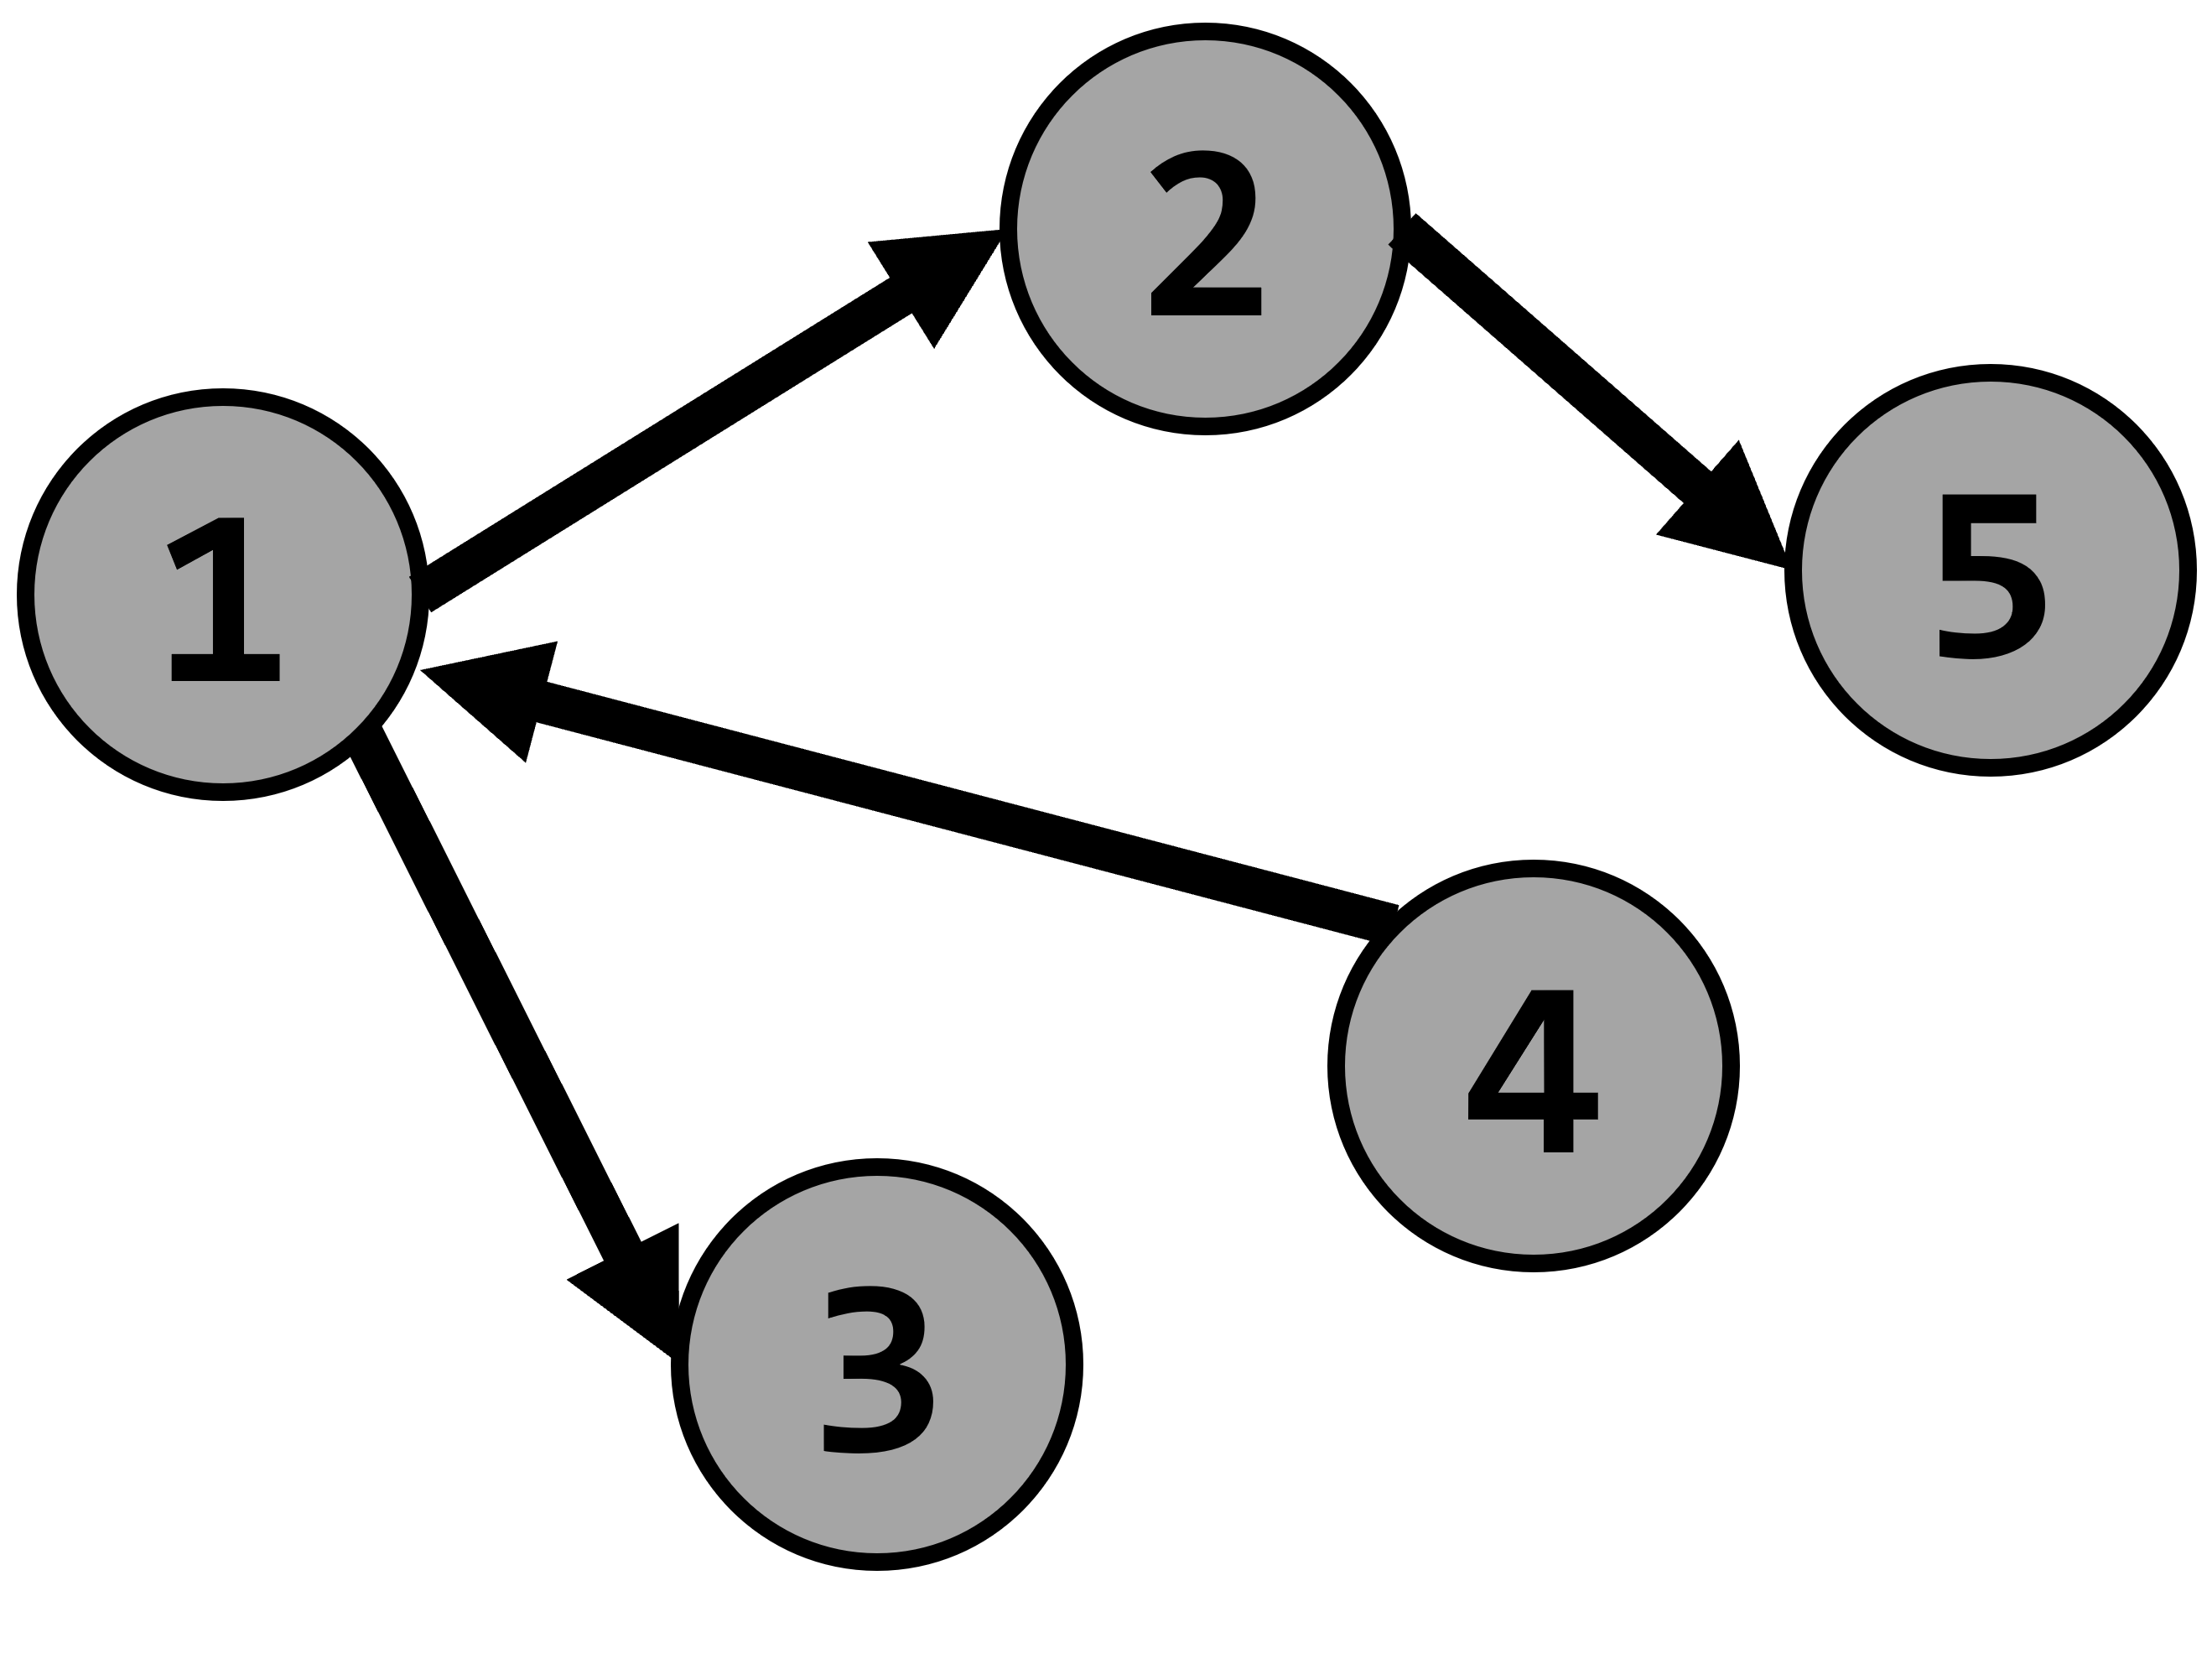
\includegraphics[scale=0.25]{grafos/dirigidos/regalos}
\end{center}

Podemos encontrar los nodos alcanzables desde el vértice 1 mediante el uso de una DFS que inicie en ese nodo. Los vértices que la DFS alcance serán aquellos donde el tesoro familiar pueda estar.


\section{Problemas de práctica}
\begin{exercise}
	\problema{Metro de la CDMX (OMI 2018)}{\omegauplink{OMI2018-Metro}}
\end{exercise}

\begin{exercise}
		\problema{Reactor (OMI 2022)}{\omegauplink{omi-2021-reactor}}
\end{exercise}